%%-----------------------------------------------------------------------------
%%
%%                                   Sean Mauch
%%                       California Institute of Technology
%%                          (a) 2000 No Rights Reserved
%%
%%-----------------------------------------------------------------------------

\flushbottom






%%=============================================================================
%%=============================================================================
\chapter{Integral Calculus}
\label{chapter_integral}
\index{integral calculus}



%%=============================================================================
\section{The Indefinite Integral}
\index{indefinite integral}

The opposite of a derivative is the \textit{anti-derivative} or the
\textit{indefinite integral}.  The indefinite integral of a function
$f(x)$ is denoted,
\[
\int f(x) \,\dd x.
\]
It is defined by the property that
\[
\frac{\dd}{\dd x} \int f(x) \,\dd x = f(x).
\]
While a function $f(x)$ has a unique derivative if it is differentiable, it
has an infinite number of indefinite integrals, each of which differ by
an additive constant.

\paragraph{Zero Slope Implies a Constant Function.}
If the value of a function's derivative is identically zero, 
$\frac{\dd f}{\dd x} = 0$, then the function is a constant, $f(x) = c$.
To prove this, we assume that there exists a non-constant differentiable
function whose derivative is zero and obtain a contradiction.  Let
$f(x)$ be such a function.  Since $f(x)$ is non-constant, there exist
points $a$ and $b$ such that $f(a) \neq f(b)$.  By the Mean Value 
Theorem of differential calculus, there exists a point $\xi \in (a,b)$
such that
\[
f'(\xi) = \frac{f(b) - f(a)}{b-a} \neq 0,
\]
which contradicts that the derivative is everywhere zero.


\paragraph{Indefinite Integrals Differ by an Additive Constant.}
Suppose that $F(x)$ and $G(x)$ are indefinite integrals of $f(x)$.  Then
we have
\[
\frac{\dd}{\dd x} (F(x) - G(x)) = F'(x) - G'(x) = f(x) - f(x) = 0.
\]
Thus we see that $F(x) - G(x) = c$ and the two indefinite integrals must
differ by a constant.  For example, we have $\int \sin x \,\dd x = - \cos x + c$.
While every function that can be expressed in terms of elementary functions,
(the exponent, logarithm, trigonometric functions, etc.), has a derivative
that can be written explicitly in terms of elementary functions, the same
is not true of integrals.  For example, $\int \sin(\sin x) \,\dd x$ cannot
be written explicitly in terms of elementary functions.



\paragraph{Properties.}
Since the derivative is linear, so is the indefinite integral.  That is,
\[
\int ( a f(x) + b g(x) ) \,\dd x = a \int f(x) \,\dd x + b \int g(x) \,\dd x.
\]
For each derivative identity there is a corresponding integral 
identity.  Consider the power law identity, 
$\frac{\dd}{\dd x} (f(x))^a = a (f(x))^{a-1} f'(x)$.  The corresponding 
integral identity is
\[
\int (f(x))^a f'(x) \,\dd x = \frac{(f(x))^{a+1}}{a+1} + c, \quad a \neq -1,
\]
where we require that $a \neq -1$ to avoid division by zero.  From the
derivative of a logarithm, $\frac{\dd}{\dd x} \ln( f(x) ) = \frac{f'(x)}{f(x)}$,
we obtain,
\[
\int \frac{f'(x)}{f(x)} \,\dd x = \ln| f(x) | + c.
\]
Note the absolute value signs.  This is because 
$\frac{\dd}{\dd x} \ln|x| = \frac{1}{x}$ for $x \neq 0$.  In Figure~\ref{log1ox}
is a plot of $\ln|x|$ and $\frac{1}{x}$ to reinforce this.

\begin{figure}[h]
  \begin{center}
    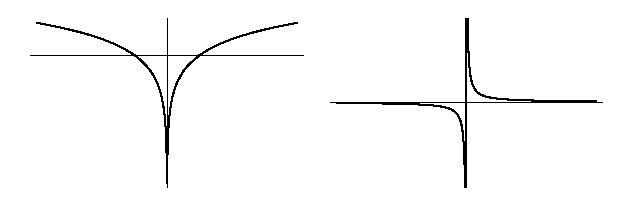
\includegraphics[width=0.5\textwidth]{calculus/integral/log1ox}
  \end{center}
  \caption{The logarithm and its derivative.}
  \label{log1ox}
\end{figure}






\begin{Example}
  Consider
  \[
  I = \int \frac{x}{(x^2 + 1)^2} \,\dd x.
  \]
  We evaluate the integral by choosing $u = x^2 + 1$, $\dd u = 2 x \,\dd x$.
  \begin{align*}
    I &= \frac{1}{2} \int \frac{2 x}{(x^2 + 1)^2} \,\dd x \\
    &= \frac{1}{2} \int \frac{\dd u}{u^2} \\
    &= \frac{1}{2} \frac{-1}{u} \\
    &= - \frac{1}{2 (x^2+1) }.
  \end{align*}
\end{Example}





\begin{Example}
  Consider
  \[
  I = \int \tan x \,\dd x = \int \frac{\sin x}{\cos x} \,\dd x.
  \]
  By choosing $f(x) = \cos x$, $f'(x) = - \sin x$, we see that the integral is
  \[
  I = - \int \frac{-\sin x}{\cos x} \,\dd x = - \ln | \cos x | + c.
  \]
\end{Example}



\paragraph{Change of Variable.}
The differential of a function $g(x)$ is $d g = g'(x) \,\dd x$.  Thus one 
might suspect that for $\xi = g(x)$, 
\begin{equation}
  \label{change_var}
  \int f(\xi) \,\dd \xi = \int f(g(x)) g'(x) \,\dd x,
\end{equation}
since $d\xi = d g = g'(x)\,\dd x$.  This turns out to be true.  To prove it
we will appeal to the the chain rule for differentiation.  Let $\xi$ be 
a function of $x$.  The chain rule is
\[
\frac{\dd}{\dd x} f(\xi) = f'(\xi) \xi'(x),
\]
\[
\frac{\dd}{\dd x} f(\xi) = \frac{\dd f}{\dd \xi} \frac{\dd \xi}{\dd x}.
\]
We can also write this as
\[
\frac{\dd f}{\dd \xi} = \frac{\dd x}{\dd \xi} \frac{\dd f}{\dd x},
\]
or in operator notation,
\[
\frac{\dd}{\dd \xi} = \frac{\dd x}{\dd \xi} \frac{\dd}{\dd x}.
\]
Now we're ready to start.  The derivative of the left side of
Equation~\ref{change_var} is
\[
\frac{\dd}{\dd \xi} \int f(\xi) \,\dd \xi = f(\xi).
\]
Next we differentiate the right side,
\begin{align*}
  \frac{\dd}{\dd \xi} \int f(g(x)) g'(x) \,\dd x
  &= \frac{\dd x}{\dd \xi} \frac{\dd}{\dd x} \int f(g(x)) g'(x) \,\dd x \\
  &= \frac{\dd x}{\dd \xi} f(g(x)) g'(x) \\
  &= \frac{\dd x}{\dd g} f(g(x)) \frac{\dd g}{\dd x} \\
  &= f(g(x)) \\
  &= f(\xi)
\end{align*}
to see that it is in fact an identity for $\xi = g(x)$.





\begin{Example}
  Consider
  \[
  \int x \sin(x^2) \,\dd x.
  \]
  We choose $\xi = x^2$, $d\xi = 2 x d x$ to evaluate the integral.
  \begin{align*}
    \int x \sin(x^2) \,\dd x
    &= \frac{1}{2} \int \sin(x^2) 2 x \,\dd x \\
    &= \frac{1}{2} \int \sin \xi \,\dd \xi \\
    &= \frac{1}{2} (-\cos \xi) + c \\
    &= - \frac{1}{2} \cos( x^2 ) + c
  \end{align*}
\end{Example}




\paragraph{Integration by Parts.}
The product rule for differentiation gives us an identity called integration
by parts.  We start with the product rule and then integrate both sides
of the equation.
\begin{gather*}
  \frac{\dd}{\dd x} (u(x) v(x)) = u'(x) v(x) + u(x) v'(x) \\
  \int ( u'(x) v(x) + u(x) v'(x) ) \,\dd x = u(x) v(x) + c \\
  \int u'(x) v(x) \,\dd x + \int u(x) v'(x) ) \,\dd x = u(x) v(x) \\
  \int u(x) v'(x) ) \,\dd x = u(x) v(x)  - \int v(x) u'(x) \,\dd x
\end{gather*}
The theorem is most often written in the form
\[
\int u \,\dd v = u v - \int v \,\dd u.
\]
So what is the usefulness of this?  Well, it may happen for some integrals
and a good choice of $u$ and $v$ that the integral on the right is easier
to evaluate than the integral on the left.



\begin{Example}
  Consider $\int x \e^x \,\dd x$.  If we choose $u = x$, $\dd v = \e^x \,\dd x$ then
  integration by parts yields
  \[
  \int x \e^x \,\dd x = x \e^x - \int \e^x \,\dd x = (x-1) \e^x.
  \]
  Now notice what happens when we choose $u = \e^x$, $\dd v = x \,\dd x$.
  \[
  \int x \e^x \,\dd x = \frac{1}{2} x^2 \e^x - \int \frac{1}{2} x^2 \e^x \,\dd x
  \]
  The integral gets harder instead of easier.
\end{Example}


When applying integration by parts, one must choose $u$ and $\dd v$
wisely.  As general rules of thumb:
\begin{itemize}
\item
  Pick $u$ so that $u'$ is simpler than $u$.
\item
  Pick $\dd v$ so that $v$ is not more complicated, (hopefully simpler), 
  than $\dd v$.
\end{itemize}
Also note that you may have to apply integration by parts several times
to evaluate some integrals.






%%=============================================================================
\section{The Definite Integral}
\index{definite integral}

%%-----------------------------------------------------------------------------
\subsection{Definition}

The area bounded by the $x$ axis, the vertical lines $x = a$ and $x = b$
and the function $f(x)$ is denoted with a \textit{definite integral}, 
\[
\int_a^b f(x) \,\dd x.
\]
The area is signed, that is, if $f(x)$ is negative, then the area is 
negative.  
We measure the area with a divide-and-conquer strategy.  
First partition the interval $(a,b)$ with
$a = x_0 < x_1 < \cdots < x_{n-1} < x_n = b$.  
Note that the area under the curve on the subinterval is approximately
the area of a rectangle of base $\Delta x_i = x_{i+1} - x_i$ and height
$f(\xi_i)$, where $\xi_i \in [x_i, x_{i+1}]$.  If we add up the areas
of the rectangles, we get an approximation of the area under the 
curve.  See Figure~\ref{intint}

\begin{figure}[h]
  \begin{center}
    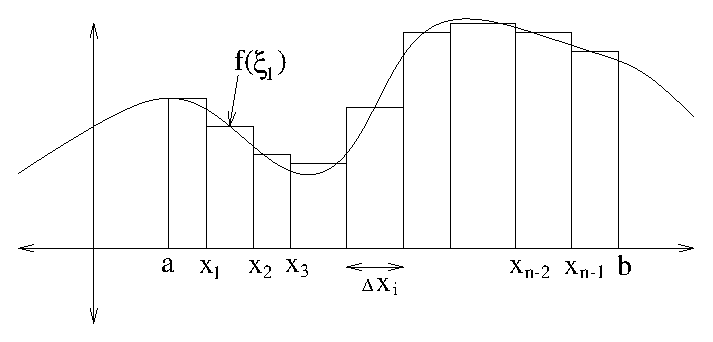
\includegraphics[width=0.6\textwidth]{calculus/integral/intint}
  \end{center}
  \caption{Divide-and-conquer strategy for approximating a definite integral.}
  \label{intint}
\end{figure}

\[
\int_a^b f(x) \,\dd x \approx \sum_{i = 0}^{n-1} f(\xi_i) \Delta x_i
\]
As the $\Delta x_i$'s get smaller, we expect the approximation of the
area to get better.  Let $\Delta x = \max_{0 \leq i \leq n-1} \Delta x_i$.
We define the definite integral as the sum of the areas of the rectangles
in the limit that $\Delta x \to 0$.
\[
\int_a^b f(x) \,\dd x 
= \lim_{\Delta x \to 0} \sum_{i = 0}^{n-1} f(\xi_i) \Delta x_i
\]
The integral is defined when the limit exists.  This is known as the
\textit{Riemann integral} of $f(x)$.  $f(x)$ is called the \textit{integrand}.




%%-----------------------------------------------------------------------------
\subsection{Properties}

\paragraph{Linearity and the Basics.}
Because summation is a linear operator, that is
\[
\sum_{i=0}^{n-1} (c f_i + d g_i) 
= c \sum_{i=0}^{n-1} f_i + d \sum_{i=0}^{n-1} g_i,
\]
definite integrals are linear,
\[
\int_a^b (c f(x) + d g(x))\,\dd x = c \int_a^b f(x)\,\dd x + d \int_a^b g(x) \,\dd x.
\]
One can also divide the \textit{range of integration}.
\[
\int_a^b f(x) \,\dd x = \int_a^c f(x) \,\dd x + \int_c^b f(x) \,\dd x
\]
We assume that each of the above integrals exist.  If $a \leq b$, and 
we integrate from $b$ to $a$, then each of the $\Delta x_i$ will be negative.
From this observation, it is clear that
\[
\int_a^b f(x) \,\dd x = - \int_b^a f(x) \,\dd x.
\]
If we integrate any function from a point $a$ to that same point $a$, then
all the $\Delta x_i$ are zero and 
\[
\int_a^a f(x) \,\dd x = 0.
\]





\paragraph{Bounding the Integral.}
Recall that if $f_i \leq g_i$, then
\[
\sum_{i=0}^{n-1} f_i \leq \sum_{i=0}^{n-1} g_i.
\]
Let $m = \min_{x \in [a,b]} f(x)$ and $M = \max_{x \in [a,b]} f(x)$.  Then
\[
(b-a) m = \sum_{i=0}^{n-1} m \Delta x_i 
\leq \sum_{i=0}^{n-1} f(\xi_i) \Delta x_i 
\leq \sum_{i=0}^{n-1} M \Delta x_i = (b-a) M
\]
implies that
\[
(b-a) m \leq \int_a^b f(x) \,\dd x \leq (b-a) M.
\]
Since
\[
\left| \sum_{i=0}^{n-1} f_i \right| \leq \sum_{i=0}^{n-1} |f_i|,
\]
we have
\[
\left| \int_a^b f(x) \,\dd x \right| \leq \int_a^b |f(x)| \,\dd x.
\]





\paragraph{Mean Value Theorem of Integral Calculus.}
Let $f(x)$ be continuous.  We know from above that
\[
(b-a) m \leq \int_a^b f(x) \,\dd x \leq (b-a) M.
\]
Therefore there exists a constant $c \in [m,M]$ satisfying
\[
\int_a^b f(x) \,\dd x = (b-a) c.
\]
Since $f(x)$ is continuous, there is a point $\xi \in [a,b]$ such that
$f(\xi) = c$.  Thus we see that 
\[
\int_a^b f(x) \,\dd x = (b-a) f(\xi),
\]
for some $\xi \in [a,b]$.







%%=============================================================================
\section{The Fundamental Theorem of Integral Calculus}
\index{fundamental theorem of calculus}


\paragraph{Definite Integrals with Variable Limits of Integration.}
Consider $a$ to be a constant and $x$ variable, then the function $F(x)$
defined by
\begin{equation}
  \label{int_var_limit}
  F(x) = \int_a^x f(t) \,\dd t
\end{equation}
is an anti-derivative of $f(x)$, that is $F'(x) = f(x)$.  To show this
we apply the definition of differentiation and the integral mean value
theorem.
\begin{align*}
  F'(x)
  &= \lim_{\Delta x \to 0} \frac{F(x+\Delta x) - F(x)}{\Delta x} \\
  &= \lim_{\Delta x \to 0} \frac{ \int_a^{x+\Delta x} f(t) \,\dd t
    - \int_a^x f(t)\,\dd t }{\Delta x} \\
  &= \lim_{\Delta x \to 0} \frac{ \int_x^{x+\Delta x} f(t) \,\dd t }
  {\Delta x} \\
  &= \lim_{\Delta x \to 0} \frac{ f(\xi) \Delta x }
  {\Delta x}, \qquad \xi \in [x,x+\Delta x] \\
  &= f(x)
\end{align*}




\paragraph{The Fundamental Theorem of Integral Calculus.}
Let $F(x)$ be any anti-derivative of $f(x)$.  Noting that all anti-derivatives
of $f(x)$ differ by a constant and replacing $x$ by $b$ in 
Equation~\ref{int_var_limit}, we see that there exists a constant $c$ 
such that
\[
\int_a^b f(x) \,\dd x = F(b) + c.
\]
Now to find the constant.  By plugging in $b = a$,
\[
\int_a^a f(x) \,\dd x = F(a) + c = 0,
\]
we see that $c = -F(a)$.  This gives us a result known as the 
\textit{Fundamental Theorem of Integral Calculus}.
\[
\int_a^b f(x) \,\dd x = F(b) - F(a).
\]
We introduce the notation
\[
[F(x)]_a^b \equiv F(b) - F(a).
\]



\begin{Example}
  \[
  \int_0^\pi \sin x \,\dd x = [-\cos x]_0^\pi = - \cos(\pi)+ \cos(0) = 2
  \]
\end{Example}






%%=============================================================================
\section{Techniques of Integration}
\index{integration!techniques of}





%%-----------------------------------------------------------------------------
\subsection{Partial Fractions}


A proper rational function
\[
\frac{p(x)}{q(x)} = \frac{p(x)}{(x-a)^n r(x)}
\]
Can be written in the form
\[
\frac{p(x)}{(x-\alpha)^n r(x)} = \left( \frac{a_0}{(x-\alpha)^n}
  + \frac{a_1}{(x-\alpha)^{n-1}} + \cdots + \frac{a_{n-1}}{x-\alpha}
\right) + (\cdots)
\]
where the $a_k$'s are constants and the last ellipses represents the
partial fractions expansion of the roots of $r(x)$.  The coefficients are
\[
a_k = \frac{1}{k!} \frac{d^k}{d x^k}
\left( \frac{p(x)}{r(x)} \right) \bigg|_{x=\alpha}.
\]




\begin{Example}
  Consider the partial fraction expansion of
  \[
  \frac{1+x+x^2}{(x-1)^3}.
  \]
  The expansion has the form
  \[
  \frac{a_0}{(x-1)^3} + \frac{a_1}{(x-1)^2} + \frac{a_2}{x-1}.
  \]
  The coefficients are
  \begin{align*}
    a_0     &= \frac{1}{0!} (1+x+x^2)|_{x=1} = 3, \\
    a_1     &= \frac{1}{1!} \frac{\dd}{\dd x}(1+x+x^2)|_{x=1}
    = (1+2x)|_{x=1} = 3, \\
    a_2     &= \frac{1}{2!} \frac{\dd^2}{\dd x^2}(1+x+x^2)|_{x=1}
    = \frac{1}{2} (2)|_{x=1} = 1.
  \end{align*}
  Thus we have
  \[
  \frac{1+x+x^2}{(x-1)^3} = \frac{3}{(x-1)^3} + \frac{3}{(x-1)^2}
  + \frac{1}{x-1}.
  \]
\end{Example}







\begin{Example}
  Suppose we want to evaluate 
  \[
  \int \frac{1+x+x^2}{(x-1)^3} \,\dd x.
  \]
  If we expand the integrand in a partial fraction expansion, then the integral
  becomes easy.
  \begin{align*}
    \int \frac{1+x+x^2}{(x-1)^3} \,\dd x.
    &= \int \left( \frac{3}{(x-1)^3} + \frac{3}{(x-1)^2}
      + \frac{1}{x-1} \right)\,\dd x \\
    &= - \frac{3}{2 (x-1)^2} - \frac{3}{(x-1)} + \ln(x-1)
  \end{align*}
\end{Example}







\begin{Example}
  Consider the partial fraction expansion of
  \[
  \frac{1+x+x^2}{x^2 (x-1)^2}.
  \]
  The expansion has the form
  \[
  \frac{a_0}{x^2} + \frac{a_1}{x} + \frac{b_0}{(x-1)^2} + \frac{b_1}{x-1}.
  \]
  The coefficients are
  \begin{align*}
    a_0     &= \frac{1}{0!} \left( \frac{1+x+x^2}{(x-1)^2} \right)
    \bigg|_{x=0} = 1, \\
    a_1     &= \frac{1}{1!} \frac{\dd}{\dd x}
    \left( \frac{1+x+x^2}{(x-1)^2} \right) \bigg|_{x=0}
    = \left( \frac{1+2x}{(x-1)^2}
      - \frac{2(1+x+x^2)}{(x-1)^3} \right) \bigg|_{x=0}
    = 3, \\
    b_0     &= \frac{1}{0!} \left( \frac{1+x+x^2}{x^2} \right)
    \bigg|_{x=1} = 3, \\
    b_1     &= \frac{1}{1!} \frac{\dd}{\dd x}
    \left( \frac{1+x+x^2}{x^2} \right) \bigg|_{x=1}
    = \left( \frac{1+2x}{x^2}
      - \frac{2(1+x+x^2)}{x^3} \right) \bigg|_{x=1}
    = -3,
  \end{align*}
  Thus we have
  \[
  \frac{1+x+x^2}{x^2 (x-1)^2} = \frac{1}{x^2} + \frac{3}{x}
  + \frac{3}{(x-1)^2} - \frac{3}{x-1}.
  \]
\end{Example}




If the rational function has real coefficients and the denominator
has complex roots, then you can reduce the work in finding the partial
fraction expansion with the following trick:  Let $\alpha$ and $\overline{\alpha}$
be complex conjugate pairs of roots of the denominator.
\begin{align*}
  \frac{p(x)}{(x-\alpha)^n (x- \overline{\alpha})^n r(x)}
  &= \left( \frac{a_0}{(x-\alpha)^n}
    + \frac{a_1}{(x-\alpha)^{n-1}} + \cdots + \frac{a_{n-1}}{x-\alpha}
  \right) \\
  &\quad + \left( \frac{\overline{a_0}}{(x-\overline{\alpha})^n}
    + \frac{\overline{a_1}}{(x-\overline{\alpha})^{n-1}} + \cdots
    + \frac{\overline{a_{n-1}}}{x-\overline{\alpha}} \right)
  + (\cdots)
\end{align*}
Thus we don't have to calculate the coefficients for the root at
$\overline{\alpha}$.  We just take the complex conjugate of the coefficients
for $\alpha$.






\begin{Example}
  Consider the partial fraction expansion of
  \[
  \frac{1+x}{x^2+1}.
  \]
  The expansion has the form
  \[
  \frac{a_0}{x-i} + \frac{\overline{a_0}}{x+i}
  \]
  The coefficients are
  \begin{align*}
    a_0     &= \frac{1}{0!} \left(\frac{1+x}{x+i} \right)
    \bigg|_{x=i} = \frac{1}{2}(1-i), \\
    \overline{a_0} &= \overline{ \frac{1}{2}(1-i)} = \frac{1}{2}(1+i)
  \end{align*}
  Thus we have
  \[
  \frac{1+x}{x^2+1} = \frac{1-i}{2(x-i)} + \frac{1+i}{2(x+i)}.
  \]
\end{Example}











%%=============================================================================
\section{Improper Integrals}
\index{improper integrals}
\index{integrals!improper}


If the range of integration is infinite or $f(x)$ is discontinuous at 
some points then $\int_a^b f(x) \,\dd x$ is called an \textit{improper
  integral}.  


\paragraph{Discontinuous Functions.}
If $f(x)$ is continuous on the interval $a \leq x \leq b$ 
except at the point $x=c$ where $a < c < b$ then
\[
\int_a^b f(x)\,\dd x = \lim_{\delta \to 0^+} \int_a^{c-\delta} f(x)\,\dd x
+ \lim_{\epsilon \to 0^+} \int_{c+\epsilon}^b f(x)\,\dd x
\]
provided that both limits exist.


\begin{Example}
  Consider the integral of $\ln x$ on the interval $[0,1]$.  Since the logarithm
  has a singularity at $x = 0$, this is an improper integral.  We write the
  integral in terms of a limit and evaluate the limit with L'Hospital's rule.
  \begin{align*}
    \int_0^1 \ln x \,\dd x
    &= \lim_{\delta \to 0} \int_\delta^1 \ln x \,\dd x \\
    &= \lim_{\delta \to 0} [x \ln x - x]_\delta^1 \\
    &= 1 \ln(1) - 1 - \lim_{\delta \to 0} (\delta \ln \delta - \delta )\\
    &= -1 - \lim_{\delta \to 0} (\delta \ln \delta ) \\
    &= -1 - \lim_{\delta \to 0} \left( \frac{ \ln \delta }{1/\delta } 
    \right) \\
    &= -1 - \lim_{\delta \to 0} \left( \frac{ 1 / \delta }{-1/\delta^2 } 
    \right) \\
    &= -1
  \end{align*}
\end{Example}




\begin{Example}
  Consider the integral of $x^a$ on the range $[0,1]$.  If $a < 0$ then there
  is a singularity at $x = 0$.  First assume that $a \neq -1$.
  \begin{align*}
    \int_0^1 x^a \,\dd x
    &= \lim_{\delta \to 0^+} \left[ \frac{x^{a+1}}{a+1} \right]_\delta^1 \\
    &= \frac{1}{a+1} - \lim_{\delta \to 0^+} \frac{\delta^{a+1}}{a+1} 
  \end{align*}
  This limit exists only for $a > -1$.  Now consider the case that $a = -1$.
  \begin{align*}
    \int_0^1 x^{-1} \,\dd x
    &= \lim_{\delta \to 0^+} \left[ \ln x \right]_\delta^1 \\
    &= \ln(0) - \lim_{\delta \to 0^+} \ln \delta
  \end{align*}
  This limit does not exist.  We obtain the result,
  \[
  \int_0^1 x^a \,\dd x = \frac{1}{a+1}, \quad \mathrm{for}\ a > -1.
  \]
\end{Example}



\paragraph{Infinite Limits of Integration.}
If the range of integration is infinite, say $[a,\infty)$ then we define
the integral as
\[
\int_a^\infty f(x) \,\dd x = \lim_{\alpha \to \infty} \int_a^\alpha f(x) \,\dd x,
\]
provided that the limit exists.
If the range of integration is $(-\infty,\infty)$ then
\[
\int_{-\infty}^\infty f(x)\,\dd x = \lim_{\alpha \to -\infty} \int_\alpha^a f(x)\,\dd x
+ \lim_{\beta \to +\infty} \int_a^\beta f(x)\,\dd x.
\]



\begin{Example}
  \begin{align*}
    \int_1^\infty \frac{\ln x}{x^2} \,\dd x
    &= \int_1^\infty \ln x \left( \frac{\dd}{\dd x} \frac{-1}{x} \right) 
    \,\dd x \\
    &= \left[ \ln x \frac{-1}{x} \right]_1^\infty 
    - \int_1^\infty \frac{-1}{x} \frac{1}{x} \,\dd x \\
    &= \lim_{x \to +\infty} \left( - \frac{ \ln x }{x} \right) 
    - \left[ \frac{1}{x} \right]_1^\infty \\
    &= \lim_{x \to +\infty} \left( - \frac{ 1/x }{1} \right) 
    - \lim_{x \to \infty} \frac{1}{x} + 1 \\
    &= 1
  \end{align*}
\end{Example}






\begin{Example}
  Consider the integral of $x^a$ on $[1,\infty)$.  First assume that
  $a \neq -1$.
  \begin{align*}
    \int_1^\infty x^a \,\dd x
    &= \lim_{\beta \to +\infty} \left[ \frac{x^{a+1}}{a+1} 
    \right]_1^\beta \\
    &= \lim_{\beta \to +\infty} \frac{\beta^{a+1}}{a+1} - \frac{1}{a+1}
  \end{align*}
  The limit exists for $\beta < -1$.  Now consider the case $a = -1$.
  \begin{align*}
    \int_1^\infty x^{-1} \,\dd x
    &= \lim_{\beta \to +\infty} \left[ \ln x
    \right]_1^\beta \\
    &= \lim_{\beta \to +\infty} \ln \beta - \frac{1}{a+1}
  \end{align*}
  This limit does not exist.  Thus we have 
  \[
  \int_1^\infty x^a \,\dd x = - \frac{1}{a+1}, \quad \mathrm{for}\ a < -1.
  \]
\end{Example}









\raggedbottom
%%=============================================================================
\pagebreak
\flushbottom
\section{Exercises}



%%-----------------------------------------------------------------------------
\begin{large}
  \noindent
  \textbf{The Indefinite Integral}
\end{large}


\begin{Exercise}[mathematica/calculus/integral/fundamental.nb]
  \label{exercise int 2x+3 10}
  Evaluate $\int (2x+3)^{10} \,\dd x$.

  \hintsolution{int 2x+3 10}
\end{Exercise}




\begin{Exercise}[mathematica/calculus/integral/fundamental.nb]
  \label{exercise int ln x 2 / x}
  Evaluate $\int \frac{(\ln x)^2}{x} \,\dd x$.

  \hintsolution{int ln x 2 / x}
\end{Exercise}



\begin{Exercise}[mathematica/calculus/integral/fundamental.nb]
  \label{exercise int x sqrt x2+3}
  Evaluate $\int x \sqrt{x^2+3}\,\dd x$.

  \hintsolution{int x sqrt x2+3}
\end{Exercise}



\begin{Exercise}[mathematica/calculus/integral/fundamental.nb]
  \label{exercise int cos x / sin x}
  Evaluate $\int \frac{\cos x}{\sin x}\,\dd x$.

  \hintsolution{int cos x / sin x}
\end{Exercise}



\begin{Exercise}[mathematica/calculus/integral/fundamental.nb]
  \label{exercise int x2 / x3-5}
  Evaluate $\int \frac{x^2}{x^3-5}\,\dd x$.

  \hintsolution{int x2 / x3-5}
\end{Exercise}



%%-----------------------------------------------------------------------------
\begin{large}
  \noindent
  \textbf{The Definite Integral}
\end{large}


\begin{Exercise}[mathematica/calculus/integral/definite.nb]
  \label{exercise int by sum x}
  Use the result
  \[
  \int_a^b f(x)\,\dd x = \lim_{N \to \infty} \sum_{n=0}^{N-1} f(x_n) \Delta x
  \]
  where $\Delta x = \frac{b-a}{N}$ and $x_n = a + n \Delta x$, to show that
  \[
  \int_0^1 x \,\dd x = \frac{1}{2}.
  \]

  \hintsolution{int by sum x}
\end{Exercise}



\begin{Exercise}[mathematica/calculus/integral/definite.nb]
  \label{exercise int 0 pi sin2 x}
  Evaluate the following integral using integration by parts and the 
  Pythagorean identity.
  $\int_0^\pi \sin^2 x \,\dd x$

  \hintsolution{int 0 pi sin2 x}
\end{Exercise}



\begin{Exercise}[mathematica/calculus/integral/definite.nb]
  \label{exercise d/dx int g f h}
  Prove that
  \[
  \frac{\dd}{\dd x} \int_{g(x)}^{f(x)} h(\xi) \,\dd \xi = h(f(x))f'(x) - h(g(x))g'(x).
  \]
  (Don't use the limit definition of differentiation, use the Fundamental
  Theorem of Integral Calculus.)

  \hintsolution{d/dx int g f h}
\end{Exercise}







\begin{Exercise}[mathematica/calculus/integral/definite.nb]
  \label{exercise area x xn}
  Let $A_n$ be the area between the curves $x$ and $x_n$ on the interval
  $[0 \ldots 1]$.  What is $\lim_{n \to \infty} A_n$?  Explain this result geometrically.

  \hintsolution{area x xn}
\end{Exercise}




\begin{Exercise}[mathematica/calculus/integral/taylor.nb]
  \label{exercise taylor series integral}
  \renewcommand{\theenumi}{\alph{enumi}}
  \begin{enumerate}
  \item
    Show that
    \[
    f(x) = f(0) + \int_0^x f'(x-\xi)\,\dd \xi.
    \]
  \item
    From the above identity show that
    \[
    f(x) = f(0) + x f'(0) + \int_0^x \xi f''(x-\xi)\,\dd \xi.
    \]
  \item
    Using induction, show that
    \[
    f(x) = f(0) + x f'(0) + \frac{1}{2} x^2 f''(0) + \cdots +
    \frac{1}{n!} x^n f^{(n)}(0)
    + \int_0^x \frac{1}{n!} \xi^n  f^{(n+1)}(x-\xi)\,\dd \xi.
    \]
  \end{enumerate}
  \renewcommand{\theenumi}{\arabic{enumi}}

  \hintsolution{taylor series integral}
\end{Exercise}



\begin{Exercise}
  \label{exercise arclength 0 x 2x}
  Find a function $f(x)$ whose arc length from $0$ to $x$ is $2 x$.

  \hintsolution{arclength 0 x 2x}
\end{Exercise}








\begin{Exercise}
  \label{exercise bounded -1 1 length}
  Consider a curve $C$, bounded by $-1$ and $1$, on the interval
  $(-1 \ldots 1)$.  Can the length of $C$ be unbounded?  What if we change
  to the closed interval $[-1 \ldots 1]$?

  \hintsolution{bounded -1 1 length}
\end{Exercise}








%%-----------------------------------------------------------------------------
\begin{large}
  \noindent
  \textbf{The Fundamental Theorem of Integration}
\end{large}


%%-----------------------------------------------------------------------------
\begin{large}
  \noindent
  \textbf{Techniques of Integration}
\end{large}


\begin{Exercise}[mathematica/calculus/integral/parts.nb]
  \label{exercise int x sin x}
  Evaluate $\int x \sin x \,\dd x$.

  \hintsolution{int x sin x}
\end{Exercise}



\begin{Exercise}[mathematica/calculus/integral/parts.nb]
  \label{exercise int x3 e2x}
  Evaluate $\int x^3 \e^{2x} \,\dd x$.

  \hintsolution{int x3 e2x}
\end{Exercise}




\begin{Exercise}[mathematica/calculus/integral/partial.nb]
  \label{exercise int 1 / x2-4}
  Evaluate $\int \frac{1}{x^2-4}\,\dd x$.

  \hintsolution{int 1 / x2-4}
\end{Exercise}





\begin{Exercise}[mathematica/calculus/integral/partial.nb]
  \label{exercise int x+1 / x3+x2-6x}
  Evaluate $\int \frac{x+1}{x^3+x^2-6x} \,\dd x$.

  \hintsolution{int x+1 / x3+x2-6x}
\end{Exercise}







%%-----------------------------------------------------------------------------
\begin{large}
  \noindent
  \textbf{Improper Integrals}
\end{large}



\begin{Exercise}[mathematica/calculus/integral/improper.nb]
  \label{exercise int 0 4 1 / (x-1)2}
  Evaluate $\int_0^4 \frac{1}{(x-1)^2} \,\dd x$.

  \hintsolution{int 0 4 1 / (x-1)2}
\end{Exercise}




\begin{Exercise}[mathematica/calculus/integral/improper.nb]
  \label{exercise int 0 1 1 / sqrt x}
  Evaluate $\int_0^1 \frac{1}{\sqrt{x}} \,\dd x$.

  \hintsolution{int 0 1 1 / sqrt x}
\end{Exercise}




\begin{Exercise}[mathematica/calculus/integral/improper.nb]
  \label{exercise int 0 infty 1 / x2+4}
  Evaluate $\int_0^\infty \frac{1}{x^2+4} \,\dd x$.

  \hintsolution{int 0 infty 1 / x2+4}
\end{Exercise}












\raggedbottom
%%=============================================================================
\pagebreak
\flushbottom
\section{Hints}



%%-----------------------------------------------------------------------------
%% The Indefinite Integral


\begin{Hint}
  \label{hint int 2x+3 10}
  Make the change of variables $u = 2 x+3$.
\end{Hint}


\begin{Hint}
  \label{hint int ln x 2 / x}
  Make the change of variables $u = \ln x$.
\end{Hint}



\begin{Hint}
  \label{hint int x sqrt x2+3}
  Make the change of variables $u = x^2 + 3$.
\end{Hint}


\begin{Hint}
  \label{hint int cos x / sin x}
  Make the change of variables $u = \sin x$.
\end{Hint}


\begin{Hint}
  \label{hint int x2 / x3-5}
  Make the change of variables $u = x^3 - 5$.
\end{Hint}




%%-----------------------------------------------------------------------------
%% The Definite Integral


\begin{Hint}
  \label{hint int by sum x}
  \begin{align*}
    \int_0^1 x \,\dd x
    &= \lim_{N \to \infty} \sum_{n=0}^{N-1} x_n \Delta x \\
    &= \lim_{N \to \infty} \sum_{n=0}^{N-1} (n \Delta x) \Delta x 
  \end{align*}
\end{Hint}



\begin{Hint}
  \label{hint int 0 pi sin2 x}
  Let $u=\sin x$ and $\dd v = \sin x \,\dd x$.  Integration by parts will give you
  an equation for $\int_0^\pi \sin^2 x \,\dd x$.
\end{Hint}





\begin{Hint}
  \label{hint d/dx int g f h}
  Let $H'(x) = h(x)$ and evaluate the integral in terms of $H(x)$.
\end{Hint}






\begin{Hint}
  \label{hint area x xn}
  CONTINUE
\end{Hint}



\begin{Hint}
  \label{hint taylor series integral}
  \renewcommand{\theenumi}{\alph{enumi}}
  \begin{enumerate}
    %%- - - - - - - - - - - - - - - - - - - - - - - - - - - - - - - - - - - 
  \item
    Evaluate the integral.
    %%- - - - - - - - - - - - - - - - - - - - - - - - - - - - - - - - - - - 
  \item
    Use integration by parts to evaluate the integral.
    %%- - - - - - - - - - - - - - - - - - - - - - - - - - - - - - - - - - - 
  \item
    Use integration by parts with $u = f^{(n+1)}(x-\xi)$ and 
    $\dd v = \frac{1}{n!} \xi^n$.
  \end{enumerate}
  \renewcommand{\theenumi}{\arabic{enumi}}
\end{Hint}



\begin{Hint}
  \label{hint arclength 0 x 2x}
  The arc length from $0$ to $x$ is
  \begin{equation}
    \label{equation int 0 x sqrt 1 + f'2}
  \int_0^x \sqrt{1 + (f'(\xi))^2} \,\dd \xi
  \end{equation}
  First show that the arc length of $f(x)$ from $a$ to $b$ is $2 (b - a)$.
  Then conclude that the integrand in 
  Equation~\ref{equation int 0 x sqrt 1 + f'2}
  must everywhere be $2$.
\end{Hint}







\begin{Hint}
  \label{hint bounded -1 1 length}
  CONTINUE
\end{Hint}


%%-----------------------------------------------------------------------------
%% The Fundamental Theorem of Integration


%%-----------------------------------------------------------------------------
%% Techniques of Integration



\begin{Hint}
  \label{hint int x sin x}
  Let $u=x$, and $\dd v = \sin x \,\dd x$.  
\end{Hint}




\begin{Hint}
  \label{hint int x3 e2x}
  Perform integration by parts three successive times.  For the first one 
  let $u = x^3$ and $\dd v = \e^{2x}\,\dd x$.  
\end{Hint}



\begin{Hint}
  \label{hint int 1 / x2-4}
  Expanding the integrand in partial fractions,
  \[
  \frac{1}{x^2-4} = \frac{1}{(x-2)(x+2)} = \frac{a}{(x-2)} + \frac{b}{(x+2)}
  \]
  \[
  1 = a (x+2) + b (x-2)
  \]
  Set $x=2$ and $x = -2$ to solve for $a$ and $b$.
\end{Hint}



\begin{Hint}
  \label{hint int x+1 / x3+x2-6x}
  Expanding the integral in partial fractions,
  \[
  \frac{x+1}{x^3+x^2-6x} = \frac{x+1}{x(x-2)(x+3)}
  = \frac{a}{x} + \frac{b}{x-2} + \frac{c}{x+3}
  \]
  \[
  x+1 = a (x-2)(x+3) + b x(x+3) + c x(x-2)
  \]
  Set $x=0$, $x=2$ and $x=-3$ to solve for $a$, $b$ and $c$.
\end{Hint}







%%-----------------------------------------------------------------------------
%% Improper Integrals


\begin{Hint}
  \label{hint int 0 4 1 / (x-1)2}
  \[
  \int_0^4 \frac{1}{(x-1)^2} \,\dd x
  = \lim_{\delta \to 0^+} \int_0^{1-\delta}
  \frac{1}{(x-1)^2} \, \dd x +
  \lim_{\epsilon \to 0^+} \int_{1+\epsilon}^4
  \frac{1}{(x-1)^2} \, \dd x
  \] 
\end{Hint}



\begin{Hint}
  \label{hint int 0 1 1 / sqrt x}
  \[
  \int_0^1 \frac{1}{\sqrt{x}} \,\dd x
  = \lim_{\epsilon \to 0^+} \int_\epsilon^1 \frac{1}{\sqrt{x}} \,\dd x 
  \]
\end{Hint}




\begin{Hint}
  \label{hint int 0 infty 1 / x2+4}
  \[
  \int \frac{1}{x^2 + a^2} \,\dd x = \frac{1}{a} \arctan \left( \frac{x}{a} \right)
  \]
\end{Hint}








\raggedbottom
%%=============================================================================
\pagebreak
\flushbottom
\section{Solutions}


%%-----------------------------------------------------------------------------
%% The Indefinite Integral



\begin{Solution}
  \label{solution int 2x+3 10}
  \[
  \int (2x+3)^{10} \,\dd x
  \]
  Let $u=2x+3$, $g(u) = x = \frac{u-3}{2}$, $g'(u) = \frac{1}{2}$.
  \begin{align*}
    \int (2x+3)^{10} \,\dd x
    &= \int u^{10} \frac{1}{2} \,\dd u \\
    &= \frac{u^{11}}{11} \frac{1}{2} \\
    &= \frac{(2x+3)^{11}}{22}
  \end{align*}
\end{Solution}



\begin{Solution}
  \label{solution int ln x 2 / x}
  \begin{align*}
    \int \frac{(\ln x)^2}{x} \,\dd x
    &= \int (\ln x)^2 \frac{\dd (\ln x)}{\dd x}\,\dd x \\
    &= \frac{(\ln x)^3}{3}
  \end{align*}
\end{Solution}



\begin{Solution}
  \label{solution int x sqrt x2+3}
  \begin{align*}
    \int x \sqrt{x^2 +3} \,\dd x
    &= \int \sqrt{x^2 + 3} \frac{1}{2} \frac{\dd (x^2)}{\dd x} \,\dd x \\
    &= \frac{1}{2} \frac{(x^2+3)^{3/2}}{3/2} \\
    &= \frac{(x^2+3)^{3/2}}{3}
  \end{align*}
\end{Solution}




\begin{Solution}
  \label{solution int cos x / sin x}
  \begin{align*}
    \int \frac{\cos x}{\sin x} \,\dd x
    &= \int \frac{1}{\sin x} \frac{\dd (\sin x)}{\dd x} \,\dd x \\
    &= \ln| \sin x |
  \end{align*}
\end{Solution}


\begin{Solution}
  \label{solution int x2 / x3-5}
  \begin{align*}
    \int \frac{x^2}{x^3 - 5} \,\dd x
    &= \int \frac{1}{x^3 - 5} \frac{1}{3}\frac{\dd (x^3)}{\dd x} \,\dd x \\
    &= \frac{1}{3} \ln | x^3 - 5 |
  \end{align*}
\end{Solution}





%%-----------------------------------------------------------------------------
%% The Definite Integral


\begin{Solution}
  \label{solution int by sum x}
  \begin{align*}
    \int_0^1 x \,\dd x
    &= \lim_{N \to \infty} \sum_{n=0}^{N-1} x_n \Delta x \\
    &= \lim_{N \to \infty} \sum_{n=0}^{N-1} (n \Delta x) \Delta x \\
    &= \lim_{N \to \infty} \Delta x^2 \sum_{n=0}^{N-1} n \\
    &= \lim_{N \to \infty} \Delta x^2 \frac{N(N-1)}{2} \\
    &= \lim_{N \to \infty} \frac{N(N-1)}{2N^2} \\
    &= \frac{1}{2}
  \end{align*}
\end{Solution}



\begin{Solution}
  \label{solution int 0 pi sin2 x}
  Let $u=\sin x$ and $\dd v = \sin x \,\dd x$.  Then $\dd u = \cos x \,\dd x$ and
  $v = -\cos x$.
  \begin{align*}
    \int_0^\pi \sin^2 x \,\dd x
    &= \big[ -\sin x \cos x \big]_0^\pi + \int_0^\pi \cos^2 x \,\dd x \\
    &= \int_0^\pi \cos^2 x \,\dd x \\
    &= \int_0^\pi (1-\sin^2 x) \,\dd x \\
    &= \pi - \int_0^\pi \sin^2 x \,\dd x
  \end{align*}
  \[
  2 \int_0^\pi \sin^2 x \,\dd x = \pi
  \]
  \[
  \int_0^\pi \sin^2 x \,\dd x = \frac{\pi}{2}
  \]
\end{Solution}



\begin{Solution}
  \label{solution d/dx int g f h}
  Let $H'(x) = h(x)$.
  \begin{align*}
    \frac{\dd}{\dd x} \int_{g(x)}^{f(x)} h(\xi) \,\dd \xi
    &= \frac{\dd}{\dd x} \left( H(f(x)) - H(g(x)) \right) \\
    &= H'(f(x))f'(x) - H'(g(x))g'(x) \\
    &= h(f(x))f'(x) - h(g(x))g'(x)
  \end{align*}
\end{Solution}



\begin{Solution}
  \label{solution area x xn}
  First we compute the area for positive integer $n$.
  \[
  A_n = \int_0^1 (x - x^n) \,\dd x
  = \left[ \frac{x^2}{2} - \frac{x^{n+1}}{n+1} \right]_0^1
  = \frac{1}{2} - \frac{1}{n+1}
  \]
  Then we consider the area in the limit as $n \to \infty$.
  \[
  \lim_{n \to \infty} A_n
  = \lim_{n \to \infty} \left( \frac{1}{2} - \frac{1}{n+1} \right)
  = \frac{1}{2}
  \]
  In Figure~\ref{figure areaxxn} we plot the functions
  $x^1, x^2, x^4, x^8, \ldots, x^{1024}$.  In the limit as $n \to \infty$, $x^n$ on the interval
  $[0 \ldots 1]$ tends to the function
  \[
  \begin{cases}
    0 &0 \leq x < 1
    \\
    1 &x = 1
  \end{cases}
  \]
  Thus the area tends to the area of the right triangle with unit base and 
  height.
  \begin{figure}[h]
    \begin{center}
      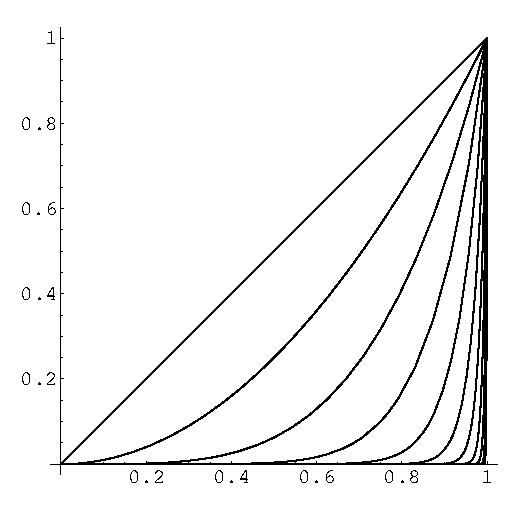
\includegraphics[width=0.4\textwidth]{calculus/integral/areaxxn}
    \end{center}
    \caption{Plots with different exponents.}
    \label{figure areaxxn}
  \end{figure}
\end{Solution}




\begin{Solution}
  \label{solution taylor series integral}
  \begin{enumerate}
  \item
    \begin{align*}
      f(0) + \int_0^x f'(x-\xi)\,\dd \xi
      &= f(0) + \left[ - f(x-\xi) \right]_0^x \\
      &= f(0) - f(0) + f(x) \\
      &= f(x)
    \end{align*}
  \item
    \begin{align*}
      f(0) + x f'(0) + \int_0^x \xi f''(x-\xi)\,\dd \xi
      &= f(0) + x f'(0) + \left[ -\xi f'(x-\xi) \right]_0^x
      - \int_0^x -f'(x-\xi) \,\dd \xi \\
      &= f(0) + x f'(0) -x f'(0)
      - \left[ f(x-\xi) \right]_0^x \\
      &= f(0) - f(0) + f(x) \\
      &= f(x)
    \end{align*}
  \item
    Above we showed that the hypothesis holds for $n=0$ and $n=1$.  Assume
    that it holds for some $n = m \geq 0$.
    \begin{align*}
      f(x)
      &= f(0) + x f'(0) + \frac{1}{2} x^2 f''(0) + \cdots +
      \frac{1}{n!} x^n f^{(n)}(0)
      + \int_0^x \frac{1}{n!} \xi^n  f^{(n+1)}(x-\xi)\,\dd \xi \\
      &= f(0) + x f'(0) + \frac{1}{2} x^2 f''(0) + \cdots +
      \frac{1}{n!} x^n f^{(n)}(0)
      + \left[ \frac{1}{(n+1)!} \xi^{n+1}
        f^{(n+1)}(x-\xi)\right]_0^x \\
      &\qquad - \int_0^x -\frac{1}{(n+1)!} \xi^{n+1}
      f^{(n+2)}(x-\xi)\,\dd \xi \\
      &= f(0) + x f'(0) + \frac{1}{2} x^2 f''(0) + \cdots +
      \frac{1}{n!} x^n f^{(n)}(0)
      + \frac{1}{(n+1)!} x^{n+1} f^{(n+1)}(0) \\
      &\qquad + \int_0^x \frac{1}{(n+1)!} \xi^{n+1}  f^{(n+2)}(x-\xi)\,\dd \xi
    \end{align*}
    This shows that the hypothesis holds for $n=m+1$.  By induction, the
    hypothesis hold for all $n \geq 0$.
  \end{enumerate}
\end{Solution}










\begin{Solution}
  \label{solution arclength 0 x 2x}
  First note that the arc length from $a$ to $b$ is $2 (b - a)$.
  \[
  \int_a^b \sqrt{1 + (f'(x))^2} \,\dd x
  = \int_0^b \sqrt{1 + (f'(x))^2} \,\dd x - \int_0^a \sqrt{1 + (f'(x))^2} \,\dd x
  = 2 b - 2 a
  \]
  Since $a$ and $b$ are arbitrary, we conclude that the integrand 
  must everywhere be $2$.
  \begin{gather*}
    \sqrt{1 + (f'(x))^2} = 2
    \\
    f'(x) = \pm \sqrt{3}
  \end{gather*}
  $f(x)$ is a continuous, piecewise differentiable function which satisfies
  $f'(x) = \pm \sqrt{3}$ at the points where it is differentiable.  One 
  example is
  \[
  \boxed{
    f(x) = \sqrt{3} x
    }
  \]
\end{Solution}










\begin{Solution}
  \label{solution bounded -1 1 length}
  CONTINUE
\end{Solution}



%%-----------------------------------------------------------------------------
%% The Fundamental Theorem of Integration


%%-----------------------------------------------------------------------------
%% Techniques of Integration



\begin{Solution}
  \label{solution int x sin x}
  Let $u=x$, and $\dd v = \sin x \,\dd x$.  Then $\dd u = \dd x$ and 
  $v = - \cos x$.
  \begin{align*}
    \int x \sin x \,\dd x
    &= -x \cos x + \int \cos x \,\dd x \\
    &= -x \cos x + \sin x + C
  \end{align*}
\end{Solution}




\begin{Solution}
  \label{solution int x3 e2x}
  Let $u = x^3$ and $\dd v = \e^{2x}\,\dd x$.  Then $\dd u = 3x^2 \,\dd x$ and
  $v = \frac{1}{2} \e^{2x}$.
  \[
  \int x^3 \e^{2x} \,\dd x = \frac{1}{2} x^3 \e^{2x} - \frac{3}{2} \int x^2 \e^{2x}\,\dd x
  \]
  Let $u = x^2$ and $\dd v = \e^{2x}\,\dd x$.  Then $\dd u = 2x \,\dd x$ and
  $v = \frac{1}{2} \e^{2x}$.
  \[
  \int x^3 \e^{2x} \,\dd x = \frac{1}{2} x^3 \e^{2x} - \frac{3}{2} \left(
    \frac{1}{2} x^2 \e^{2x} - \int x \e^{2x} \,\dd x \right)
  \]
  \[
  \int x^3 \e^{2x} \,\dd x = \frac{1}{2} x^3 \e^{2x} - \frac{3}{4} x^2 \e^{2x}
  + \frac{3}{2} \int x \e^{2x} \,\dd x
  \]
  Let $u = x$ and $\dd v = \e^{2x}\,\dd x$.  Then $\dd u = \dd x$ and
  $v = \frac{1}{2} \e^{2x}$.
  \[
  \int x^3 \e^{2x} \,\dd x = \frac{1}{2} x^3 \e^{2x} - \frac{3}{4} x^2 \e^{2x}
  + \frac{3}{2} \left( \frac{1}{2} x \e^{2x} - \frac{1}{2}
    \int \e^{2x} \,\dd x \right)
  \]
  \[
  \int x^3 \e^{2x} \,\dd x = \frac{1}{2} x^3 \e^{2x} - \frac{3}{4} x^2 \e^{2x}
  + \frac{3}{4} x \e^{2x} - \frac{3}{8} \e^{2x} + C
  \]
\end{Solution}





\begin{Solution}
  \label{solution int 1 / x2-4}
  Expanding the integrand in partial fractions,
  \[
  \frac{1}{x^2-4} = \frac{1}{(x-2)(x+2)} = \frac{A}{(x-2)} + \frac{B}{(x+2)}
  \]
  \[
  1 = A (x+2) + B (x-2)
  \]
  Setting $x=2$ yields $A = \frac{1}{4}$.  Setting $x=-2$ yields
  $B = -\frac{1}{4}$.
  Now we can do the integral.
  \begin{align*}
    \int \frac{1}{x^2-4}\,\dd x
    &= \int \left(\frac{1}{4(x-2)} - \frac{1}{4(x+2)} \right)\,\dd x \\
    &= \frac{1}{4} \ln |x-2| - \frac{1}{4} \ln |x+2| + C \\
    &= \frac{1}{4} \left| \frac{x-2}{x+2} \right| + C
  \end{align*}
\end{Solution}




\begin{Solution}
  \label{solution int x+1 / x3+x2-6x}
  Expanding the integral in partial fractions,
  \[
  \frac{x+1}{x^3+x^2-6x} = \frac{x+1}{x(x-2)(x+3)}
  = \frac{A}{x} + \frac{B}{x-2} + \frac{C}{x+3}
  \]
  \[
  x+1 = A (x-2)(x+3) + B x(x+3) + C x(x-2)
  \]
  Setting $x=0$ yields $A = -\frac{1}{6}$.
  Setting $x=2$ yields $B = \frac{3}{10}$.
  Setting $x=-3$ yields $C = -\frac{2}{15}$.
  \begin{align*}
    \int \frac{x+1}{x^3+x^2-6x} \,\dd x
    &= \int \left( - \frac{1}{6x} + \frac{3}{10(x-2)} - \frac{2}{15(x+3)}
    \right) \,\dd x \\
    &= -\frac{1}{6} \ln |x| + \frac{3}{10} \ln |x-2|
    - \frac{2}{15} \ln |x+3| + C \\
    &= \ln \frac{|x-2|^{3/10}}{|x|^{1/6} |x+3|^{2/15}} + C
  \end{align*}
\end{Solution}





%%-----------------------------------------------------------------------------
%% Improper Integrals



\begin{Solution}
  \label{solution int 0 4 1 / (x-1)2}
  \begin{align*}
    \int_0^4 \frac{1}{(x-1)^2} \,\dd x
    &= \lim_{\delta \to 0^+} \int_0^{1-\delta}
    \frac{1}{(x-1)^2} \, \dd x +
    \lim_{\epsilon \to 0^+} \int_{1+\epsilon}^4
    \frac{1}{(x-1)^2} \, \dd x \\
    &= \lim_{\delta \to 0^+} \left[-\frac{1}{x-1}\right]_0^{1-\delta} +
    \lim_{\epsilon \to 0^+}
    \left[-\frac{1}{x-1}\right]_{1+\epsilon}^4  \\
    &= \lim_{\delta \to 0^+} \left( \frac{1}{\delta} - 1 \right) +
    \lim_{\epsilon \to 0^+} \left( -\frac{1}{3} +
      \frac{1}{\epsilon} \right) \\
    &= \infty + \infty
  \end{align*}
  The integral diverges.
\end{Solution}



\begin{Solution}
  \label{solution int 0 1 1 / sqrt x}
  \begin{align*}
    \int_0^1 \frac{1}{\sqrt{x}} \,\dd x
    &= \lim_{\epsilon \to 0^+} \int_\epsilon^1 \frac{1}{\sqrt{x}} \,\dd x \\
    &= \lim_{\epsilon \to 0^+} \left[ 2 \sqrt{x}
    \right]_\epsilon^1 \\
    &= \lim_{\epsilon \to 0^+} 2 ( 1 - \sqrt{\epsilon} ) \\
    &= 2
  \end{align*}
\end{Solution}



\begin{Solution}
  \label{solution int 0 infty 1 / x2+4}
  \begin{align*}
    \int_0^\infty \frac{1}{x^2+4} \,\dd x
    &= \lim_{\alpha \to \infty} \int_0^\alpha \frac{1}{x^2+4} \,\dd x \\
    &= \lim_{\alpha \to \infty} \left[ \frac{1}{2} \arctan
      \left( \frac{x}{2} \right) \right]_0^\alpha \\
    &= \frac{1}{2} \left( \frac{\pi}{2} - 0 \right) \\
    &= \frac{\pi}{4}
  \end{align*}
\end{Solution}








\raggedbottom
%%=============================================================================
\pagebreak
\flushbottom
\section{Quiz}


\begin{QuizProblem}
  \label{quiz problem limit sum definition}
  Write the limit-sum definition of $\int_a^b f(x)\,\dd x$.

  \quizsolution{limit sum definition}
\end{QuizProblem}


\begin{QuizProblem}
  \label{quiz problem int sqrt |x|}
  Evaluate $\int_{-1}^2 \sqrt{|x|} \,\dd x$.

  \quizsolution{int sqrt |x|}
\end{QuizProblem}


\begin{QuizProblem}
  \label{quiz problem ddx int x x2 f}
  Evaluate $\frac{\dd}{\dd x} \int_x^{x^2} f(\xi) \,\dd \xi$.

  \quizsolution{ddx int x x2 f}
\end{QuizProblem}


\begin{QuizProblem}
  \label{quiz problem int 1xx2 x13}
  Evaluate $\int \frac{1+x+x^2}{(x+1)^3} \,\dd x$.

  \quizsolution{int 1xx2 x13}
\end{QuizProblem}


\begin{QuizProblem}
  \label{quiz problem integral mean value theorem}
  State the integral mean value theorem.

  \quizsolution{integral mean value theorem}
\end{QuizProblem}


\begin{QuizProblem}
  \label{quiz problem partial fraction 1xx-1x-2x-3}
  What is the partial fraction expansion of $\frac{1}{x(x-1)(x-2)(x-3)}$?

  \quizsolution{partial fraction 1xx-1x-2x-3}
\end{QuizProblem}






\raggedbottom
%%=============================================================================
\pagebreak
\flushbottom
\section{Quiz Solutions}


\begin{QuizSolution}
  \label{quiz solution limit sum definition}
  Let $a = x_0 < x_1 < \cdots < x_{n-1} < x_n = b$
  be a partition of the interval $(a..b)$.
  We define $\Delta x_i = x_{i+1} - x_i$ and $\Delta x = \max_i \Delta x_i$
  and choose $\xi_i \in [x_i .. x_{i+1}]$.
  \[
  \int_a^b f(x) \,\dd x
  = \lim_{\Delta x \to 0} \sum_{i = 0}^{n-1} f(\xi_i) \Delta x_i
  \]
\end{QuizSolution}


\begin{QuizSolution}
  \label{quiz solution int sqrt |x|}
  \begin{align*}
    \int_{-1}^2 \sqrt{|x|} \,\dd x
    &= \int_{-1}^0 \sqrt{-x}\,\dd x + \int_0^2 \sqrt{x}\,\dd x 
    \\
    &= \int_0^1 \sqrt{x}\,\dd x + \int_0^2 \sqrt{x}\,\dd x 
    \\
    &= \left[ \frac{2}{3} x^{3/2} \right]_0^1
    + \left[ \frac{2}{3} x^{3/2} \right]_0^2 
    \\
    &= \frac{2}{3} + \frac{2}{3} 2^{3/2} 
    \\
    &= \frac{2}{3} (1 + 2 \sqrt{2} )
  \end{align*}
\end{QuizSolution}


\begin{QuizSolution}
  \label{quiz solution ddx int x x2 f}
  \begin{align*}
    \frac{\dd}{\dd x} \int_x^{x^2} f(\xi) \,\dd \xi
    &= f(x^2) \frac{\dd}{\dd x}(x^2) 
    - f(x) \frac{\dd}{\dd x} (x)
    \\
    &= 2 x f(x^2) - f(x)
  \end{align*}
\end{QuizSolution}


\begin{QuizSolution}
  \label{quiz solution int 1xx2 x13}
  First we expand the integrand in partial fractions.
  \[
  \frac{1+x+x^2}{(x+1)^3} = \frac{a}{(x+1)^3} + \frac{b}{(x+1)^2}
  + \frac{c}{x+1}
  \]
  \begin{align*}
    a &= (1+x+x^2)\big|_{x=-1} = 1 
    \\
    b &= \frac{1}{1!} \left(\frac{\dd}{\dd x} (1+x+x^2) \right) \bigg|_{x=-1} 
    = \left( 1+2x\right) \big|_{x=-1}  = -1 
    \\
    c &= \frac{1}{2!} \left(\frac{\dd^2}{\dd x^2} (1+x+x^2) \right) \bigg|_{x=-1} 
    = \frac{1}{2} \left( 2 \right) \big|_{x=-1}  = 1 
  \end{align*}
  Then we can do the integration.
  \begin{align*}
    \int \frac{1+x+x^2}{(x+1)^3} \,\dd x 
    &= \int \left( \frac{1}{(x+1)^3} - \frac{1}{(x+1)^2} + \frac{1}{x+1} \right)
    \,\dd x 
    \\
    &= -\frac{1}{2 (x+1)^2} + \frac{1}{x+1} + \ln |x+1| 
    \\
    &= \frac{x + 1/2}{(x+1)^2} + \ln |x+1|
  \end{align*}
\end{QuizSolution}


\begin{QuizSolution}
  \label{quiz solution integral mean value theorem}
  Let $f(x)$ be continuous.  Then
  \[
  \int_a^b f(x) \,\dd x = (b-a) f(\xi),
  \]
  for some $\xi \in [a .. b]$.
\end{QuizSolution}


\begin{QuizSolution}
  \label{quiz solution partial fraction 1xx-1x-2x-3}
  \[
  \frac{1}{x(x-1)(x-2)(x-3)} = \frac{a}{x} + \frac{b}{x-1} + \frac{c}{x-2}
  + \frac{d}{x-3}
  \]
  \begin{align*}
    a &= \frac{1}{(0-1)(0-2)(0-3)} = - \frac{1}{6} 
    \\
    b &= \frac{1}{(1)(1-2)(1-3)} = \frac{1}{2} 
    \\
    c &= \frac{1}{(2)(2-1)(2-3)} = - \frac{1}{2} 
    \\
    d &= \frac{1}{(3)(3-1)(3-2)} = \frac{1}{6}
  \end{align*}
  \[
  \frac{1}{x(x-1)(x-2)(x-3)} = - \frac{1}{6 x} + \frac{1}{2(x-1)} 
  - \frac{1}{2(x-2)} + \frac{1}{6(x-3)}
  \]
\end{QuizSolution}







\raggedbottom

